\section{Автоколебания}
\subsection{Общие положения}

Автоколебания -- это режим диссипативной колебательной системы, в котором
установившиеся параметры колебаний не зависят от начальных условий.

Автоколебательными обычно являются нелинейные системы с трением. При этом
движение изображающей точки на фазовой плоскости может иметь и непериодический
характер. В таких случаях выделяют 2 типа автоколебаний:
\begin{itemize}
    \item квазипериодические -- их спектр содержит пару-тройку основных
        гармоник, частоты которых находятся в иррациональном соотношении; в
        результате они выглядят как периодические, но таковыми не являются;
    \item хаотические колебания -- спектр этих колебаний сплошной, при этом
        фазовая точка движется вблизи некоторой кривой (называемой аттрактором),
        неограниченно приближаясь к ней.
\end{itemize}

Рассмотрим теперь примеры автоколебательных систем.
\subsection{Примеры}

\subsubsection{Колебательный контур с нелинейной обратной связью}
\begin{figure}[h]
\begin{center}
    \begin{circuitikz}
        \draw (0,0) to[L=$L$] (0, -2);
        \draw (0,-2) to[R=$R$] (0, -4);
        \draw (0,-4) to (3, -4);
        \draw (0,0) to[short,i^=$i$] (3, 0);
        \draw (3,0) to[C=$C$,v>=$u$] (3, -4);
        \draw (-1,-.2) to[L] (-1, -1.8);
        \draw (-2,-.1) to (-2, -2);
        \draw (-2,-2) to (-3, -2);
        \draw (-3,-2) to (-3, -.1);
        \draw (-3,-.1) to (-2, -.1);
        \draw (-2.5,-.1) to (-2.5, 0);
        \draw (-2.5,0) to (0, 0);
        \draw (-2,-.2) to (-1, -.2);
        \draw (-1,-1.8) to[short,i_=$i_1$] (-2, -1.8);
        \draw (-2.5,-2) to (-2.5, -4);
        \draw (-2.5,-4) to (0, -4);
    \end{circuitikz}
\end{center}
\end{figure}

Первым примером послужит колебательный контур, который имеет индуктивную
обратную связь. Причём ток в цепи обратной связи зависит от напряжения нелинейно
\[
    i_1 = g_0u - g_1u^3.
\]
Запишем правило Кирхгофа для этого контура:
\[
    u + iR + L\der{i}{t} - M\der{i_1}{t} = 0.
\]
Так как задана зависимость \( i_1(u) \), то имеет смысл записать уравнение для
напряжения. Тогда
\[
    i = C\pder{u}{t},\quad
    u + RC\der{u}{t} + LC\dder{u}{t} - M(g_0 - 3g_1u^2)\der{u}{t} = 0,
\]
\[
    LC\dder{u}{t} + (RC - Mg_0 + 3Mg_1u^2)\der{u}{t} + u = 0.
\]
Для удобства решения этого уравнения, перейдём к новым переменным
\[
    \tau = \frac{t}{\sqrt{LC}},\quad
    x = \frac{\sqrt{3g_1M}}{\sqrt[4]{LC}}u,\quad
    \lambda = \frac{Mg_0 - RC}{\sqrt{LC}}.
\]
С этими новыми переменными уравнение примет вид:
\[
    \ddot{x} - (\lambda + x^2)\dot{x} + x = 0.
\]
Это уравнение называется уравнением Ван-дер-Поля.

\subsubsection{Брюсселятор Пригожина}
Автоколебания могут наблюдаться и в химических реакциях. Одними из первых такую
реакцию наблюдали Белоусов и Жаботинский. Сейчас под реакцией
Белоусова-Жаботинского понимают класс химических реакций, протекающих в
колебательном режиме, при котором некоторые параметры реакции (цвет,
концентрация компонентов, температура и др.) периодически изменяются.

Одной из моделей такой реакции является брюсселятор Пригожина. Он описывается
следующей последовательностью реакций:
\begin{align*}
    A      & \xrightarrow{k_1} X,\\
    X + B  & \xrightarrow{k_2} Y + D,\\
    2X + Y & \xrightarrow{k_3} 3X,\\
    X      & \xrightarrow{k_4} E.
\end{align*}
Здесь вещества A и B берутся в избытке, а колебания в концентрациях
наблюдаются для промежуточных веществ X и Y.

Для концентраций промежуточных веществ получаются дифференциальные уравнения:
\[
    \left\{
        \begin{array}{l}
            \der{[X]}{t} = k_1[A] - k_2[B][X] + k_3[X]^2[Y] - k_4[X],\\
            \der{[Y]}{t} = k_2[B][X] - k_3[X]^2[Y].\\
        \end{array}
    \right.
\]
Теперь попробуем перейти к более удобным переменным. Для начала введём
безразмерные величины для концентраций
\[
    [X] = [X]_0 x,\quad [Y] = [Y]_0 y,
\]
где \( [X]_0 \) и \( [Y]_0 \) -- равновесные концентрации, которые можно
определить, решив систему
\[
    \left\{
        \begin{array}{l}
            k_1[A] - k_2[B][X]_0 + k_3[X]_0^2[Y]_0 - k_4[X]_0 = 0,\\
            k_2[B][X]_0 - k_3[X]_0^2[Y]_0 = 0.\\
        \end{array}
    \right.
\]
Нетрудно видеть, что
\[
    [X]_0 = \frac{k_1 [A]}{k_4},\quad [Y]_0 = \frac{k_2[B]}{k_3[X]_0} =
        \frac{k_2k_4}{k_1k_3}\frac{[B]}{[A]}.
\]
Тогда уравнения можно переписать в виде
\[
    \left\{
        \begin{array}{l}
            \der{x}{t} = k_1\frac{[A]}{[X]_0} - (k_2[B] + k_4)x +
                k_3[X_0][Y_0]x^2y,\\
            \der{y}{t} = k_2\frac{[B][X]_0}{[Y]_0}x -
                k_3[X]_0^2x^2y.\\
        \end{array}
    \right.
\]
Теперь подставим выражения для \( [X]_0 \) и \( [Y]_0 \):
\[
    \left\{
        \begin{array}{l}
            \der{x}{t} = k_4 - (k_2[B] + k_4)x + k_2[B]x^2y,\\
            \der{y}{t} = \frac{k_3k_1^2}{k_4^2}[A]^2 (x - x^2y).\\
        \end{array}
    \right.
\]
Теперь стоит перейти к новой временной координате. Положим \( \tau = k_4t \) и
будем писать дифференцирование по \( \tau \) при помощи точки сверху:
\[
    \left\{
        \begin{array}{l}
            \dot{x} = 1 - (\frac{k_2[B]}{k_4} + 1)x + \frac{k_2[B]}{k_4}x^2y,\\
            \dot{y} = \frac{k_3k_1^2}{k_4^3}[A]^2 (x - x^2y).\\
        \end{array}
    \right.
\]
Введём обозначения
\[
    a = \frac{k_2[B]}{k_4},\quad b = \frac{k_3k_1^2}{k_4^3}[A]^2
\]
и перепишем систему в ещё более привлекательном виде
\[
    \left\{
        \begin{array}{l}
            \dot{x} = 1 - (a + 1)x + ax^2y,\\
            \dot{y} = b(x - x^2y).\\
        \end{array}
    \right.
\]

Исследуем устойчивость положения равновесия. Для этого линеаризуем уравнение
вблизи точки \( (1, 1) \):
\[
    x = 1 + \xi,\quad y = 1 + \eta,
\]
\[
    \left\{
        \begin{array}{l}
            \dot{\xi} = 1 - (a + 1)(1 + \xi) + a(1+\xi)^2(1+\eta),\\
            \dot{\eta} = b[(1+\xi) - (1+\xi)^2(1+\eta)].
        \end{array}
    \right.
\]
Раскроем скобки и оставим слагаемые только нулевого и первого порядков малости:
\[
    \left\{
        \begin{array}{l}
            \dot{\xi} = 1 - (a + 1)(1 + \xi) + a(1+2\xi+\eta) =
                (a-1)\xi + a\eta, \\
            \dot{\eta} = -b\xi -b\eta.
        \end{array}
    \right.
\]
Характеристическое уравнение этой системы имеет вид
\[
    \begin{vmatrix}
        a - 1 - \lambda & a           \\
        -b              & -b - \lambda
    \end{vmatrix}
    = 0,
\]
\[
    \lambda^2 - (a-1 - b) \lambda - (a-1)b + ab = 0,
\]
\[
    \lambda^2 - (a - b - 1) \lambda + b = 0,
\]
\[
    \lambda_{1,2} = \frac{a-b-1}{2} \pm \sqrt{\frac{(a-b-1)^2}{4} - b}.
\]
Рассмотрим сначала действительные решения. Они получаются при условии
\[
    |a - b - 1| > 2\sqrt{b},
\]
\[
    \left[
        \begin{array}{l}
            a - b - 1 > 2\sqrt{b},\\
            a - b - 1 < -2\sqrt{b}
        \end{array}
    \right.
\]
При этом оба действительных решения имеют один и тот же знак, определяемый
знаком \( a - b - 1 \). При \( a > (\sqrt{b} + 1)^2 \) получаем
\[
    a - b - 1 > 2\sqrt{b}
\]
и положение равновесия неустойчиво (неустойчивый узел), а при
\( a < (\sqrt{b} - 1)^2 \) -- устойчиво (устойчивый узел).

Теперь перейдём к комплексным. Они, очевидно, имеют место при
\[
    -2\sqrt{b} < a - b - 1 < 2\sqrt{b}.
\]
При этом, если \( (\sqrt{b} - 1)^2 < a < b + 1 \), то \( \Re\lambda < 0 \) и
точка является устойчивым фокусом, а в случае \( b + 1 < a < (\sqrt{b} + 1)^2 \)
-- неустойчивым фокусом.

Несмотря на возможную неустойчивость положения равновесия, у брюсселятора
существует предельный цикл. Поэтому при неустойчивом поведении вблизи точки
равновесия, система совершает автоколебания.

Фазовый портрет и временные зависимости концентраций представлены на рисунке
ниже. При расчёте использовались значения \( a = 3,\ b = 1 \).

\begin{figure}[h]
\begin{center}
    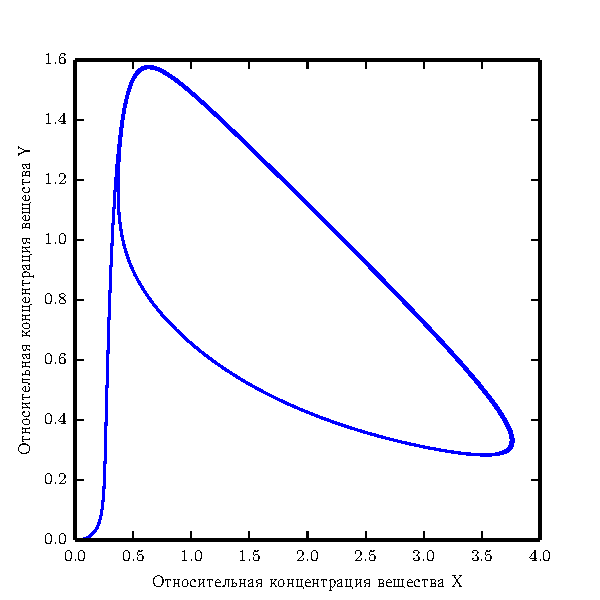
\includegraphics[width = .47\textwidth]{05-brusselator/phase_portrait}
    \hfill
    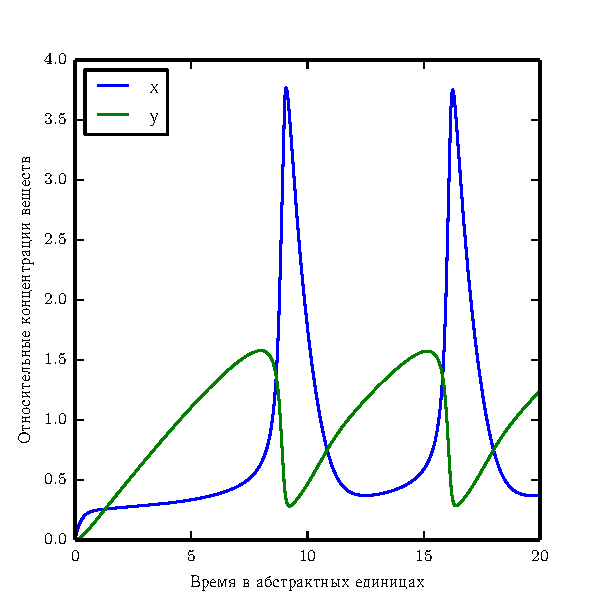
\includegraphics[width = .47\textwidth]{05-brusselator/in_time}
\end{center}
\end{figure}

